\ifx\wholebook\relax\else
\input{../Common.tex}
\input{../macroes.tex}
\begin{document}
\fi


\chapter{Fun with Robots}\label{cha:custo}

\begin{chapterfigure}
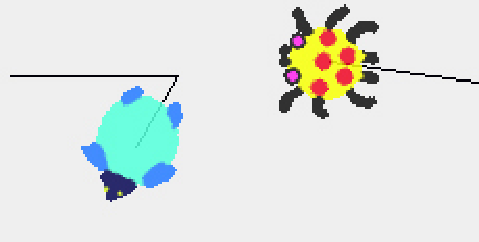
\includegraphics{beasts}
\end{chapterfigure}

The basic look of the robots is rather simple. In this chapter we show you how we can change the shape, the size and the color of robots. We present how \replace{you can draw yourselves the appearance of}{to change the way} your robots \replace{to simulate}{are drawn,} for example \add{to look like} animals.  


\section{Pen Size and Color}
So far the \replace{trace}{track} left by our robot was black. However, you can change the color of a \replace{robot}{robot's} pen \add{ by} sending it the message \ct{penColor: }\index{penColor: aColor} with a color. For example the expression \ct{\caro penColor: Color blue} changes the color of the pen to blue. \add{\paragraph
}
One of the \replace{way}{ways} to create a color is to send a message with the name of a color to the class \ct{Color} \replace{as for example}{, such as} \ct{Color blue} or \ct{Color yellow}. We will explain colors in the following section. \add{\paragraph
}
We can also change the \replace{size}{thickness} of the \replace{robot}{robot's} pen by sending the message \index{penSize:}\ct{penSize:} with a number as argument\add{, for instance} (\ct{\caro penSize: 5}). \add{\paragraph
}
\replace{The script}{Script }~\ref{scr:blueLine} draws a thick blue line\replace{ while the script}{. Script }~\ref{scr:Stair} draws a strange \replace{stair}{staircase} by \add{repeatedly} increasing \remove{regularly} the pen size.

\begin{scriptwithtitle}{A blue line}\label{scr:blueLine}
| \caro |
\caro := \Turtle new.
\caro \textbf{penColor: Color blue}.
\caro go: 100.
\caro \textbf{penSize: 5}.
\caro go: 100
\end{scriptwithtitle}


\ 


\begin{scriptfig}{turtleMPenSize}{Stair}\label{scr:Stair}
| \caro |
\caro := \Turtle new.
\caro go: 40.
\caro penSize: 2.
\caro go: 40.
\caro penSize: 4.
\caro go: 40.
\caro penSize: 6.
\caro go: 40.
\end{scriptfig}

\ 

Changing the color of the robot itself is also possible using the
method \index{color: aColor}\ct{color:} (\add{for instance }\ct{\caro color: Color yellow}). \remove{The} \scriptref{scr:yellowturtle} asks \ct{daly} to change its color\replace{, to}{and} go forward\add{,} while \caro does not move.

\begin{scriptwithtitle}{Two Robots}\label{scr:yellowturtle}
| \caro daly |
\caro := \Turtle new.
daly  := \Turtle new.
daly color: Color yellow.
daly go: 100.
\end{scriptwithtitle}

\section{About Colors}

As mentioned already, \sq  is an environment built from and using objects. Therefore programming in \sq amounts to \replace{create}{creating} objects and \replace{send}{sending} them messages. In particular a \emph{color} is an object created by the class \ct{Color}. To get a color you \remove{should} send a message to the class \ct{Color}. \add{\paragraph
}

\add{Some color messages are named for the color they get.} For example, \ct{Color red} creates the color red. Here is the list of the predefined \add{color name} messages that you can send \remove{to create a color} to the class \ct{Color} \add{to create that color}: 
\ct{black}, \ct{veryVeryDarkGray}, \ct{veryDarkGray}, \ct{darkGray}, \ct{gray}, \ct{lightGray}, \ct{veryLightGray}, \ct{veryVeryLightGray}, \ct{white}, \ct{red}, \ct{yellow}, \ct{green}, \ct{cyan}, \ct{blue}, \ct{magenta}, \ct{brown}, \ct{orange}, \ct{lightRed}, \ct{lightYellow}, \ct{lightGreen}, \ct{lightCyan}, \ct{lightBlue}, \ct{lightMagenta}, \ct{lightBrown}, \ct{lightOrange}, \ct{paleBuff}, \ct{paleBlue}, \ct{paleYellow}, \ct{paleGreen} ,\ct{paleRed}, \ct{veryPaleRed}, \ct{paleTan}, \ct{paleMagenta}, \ct{paleOrange}, and \ct{palePeach}.

@@dank: effect of \Tscrref vs \scrref?@@ \add{You can also make a color by telling the \ct{Color} factory how to make it by mixing red, green and blue.}  \Tscrref{scr:colorCreation} shows how to create colors \replace{explicitly}{this way} using the \replace{methods}{method} \index{r:g:b:}\ct{r: red g: green b: blue}\remove{ and \index{h:s:v:}\ct{h: hue s: saturation v: brightness}}. @@dank: I recommend not mentioning h:s:v: unless you want to spend a few paragraphs explaining it.@@ The arguments of \replace{the methods \ct{h:s:v:} and}{method} \ct{r:g:b:} should be \replace{float}{decimal} numbers \replace{ranged from}{between} 0 \replace{to}{and} 1.0. For example the expression \ct{Color r: 1 g:0 b:0} creates the \replace{color}{same pure} red \replace{equivalent to}{color that you get from} \ct{Color red}. \newcomma
 nd{\add}[1]{\paragraph
}
Finally the method \index{fromUser}\ct{fromUser} \replace{allows}{lets} you \replace{to choose directly}{pick} a color \add{from a palette on the screen,} and \replace{show}{then shows} you \replace{the color}{that color's} ingredients. For that you need to execute the expression \ct{Color fromUser} using the \menu{print it} menu to get the result of the selection printed.

Print the result by using the \replace{print it}{\menu{print it}} menu when executing the expression \ct{Color fromUser}).

\begin{scriptfig}{colorFromUser}{Other ways to create colors}\label{scr:colorCreation}
"Produce a pure red"
Color h: 0 s: 1 v: 1
Color r: 1 g:0 b:0

"To choose your color \replace{direclty}{from a picture}"
Color fromUser
\end{scriptfig}



\section{Changing Robot Shape}
\fprod{this section will change}
Another aspect of a robot that you can change is its shape. Two different shapes \add{--} a circle\add{,} and a triangle \add{--} are \replace{proposed by default plus}{built into the \ct{Bot} factory. \sq also has} the \replace{possibility}{ability} to \replace{draw}{add} your own \replace{shape}{shapes,} as shown later in Section~\ref{sec:drawingTurtle}.

\begin{figure}[h]
\begin{center}
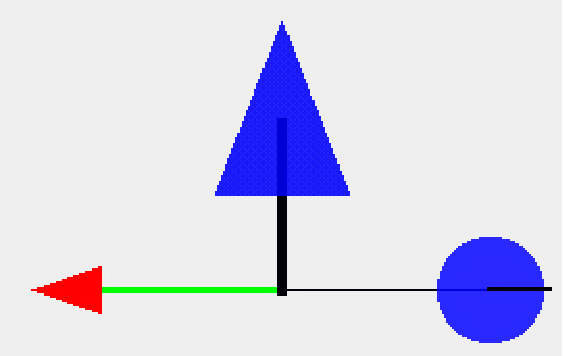
\includegraphics[width=8cm]{shapeAndSize}
\caption{Different robot shapes and \replace{size}{sizes}. \label{fig:shapeAndSize}}
\end{center}
\end{figure}

\Tscrref{scr:differentsize} shows how to change the shape of a robot \remove{using the message \index{lookLikeTriangle} \ct{lookLikeTriangle}} as shown in Figure~\ref{fig:shapeAndSize}. \add{The message \index{lookLikeTriangle} \ct{lookLikeTriangle} gives the triangular robot.} The default shape, the circle, is produced by sending the message   \index{lookLikeCircle} \ct{lookLikeCircle}. 

\begin{scriptwithtitle}{Creating Robots of Different \replace{Size}{Sizes} and \replace{Shape}{Shapes}}\label{scr:differentsize}
| \caro daly  big\caro |
\caro := \Turtle new.
\caro \textbf{lookLikeTriangle}.
\caro west.
\caro color: Color red.
\caro penColor: Color green.
\caro penSize: 3.
\caro go: 100.
daly := \Turtle new.
daly \textbf{extent: 60@60}.
daly east.
daly go: 100.
big\caro := \Turtle new.
big\caro \textbf{lookLikeTriangle}.
big\caro \textbf{extent: 100@150}.
big\caro penSize: 5.
big\caro north.
big\caro go: 80.
\end{scriptwithtitle}


\paragraph{Robot Size.}@@dank: Would you consider renaming the argument 'aPoint' to something more understandable, such as 'widthAndHeight'?  This would avoid some confusion and allow putting off any discussion of 'point' until later.@@
The second aspect you can change is the size of a robot using the message \index{extent:} \ct{extent: aPoint}, where the values of the point represent the width and height of the rectangle in which the robot is drawn. A point is composed of two numbers separated by the \ct{@} symbol. For example, the point \ct{50@100} represents a rectangle of 50 pixels \replace{on}{by} 100.







\section{Drawing Your Own Robot}\label{sec:drawingTurtle}
\fprod{this section will change:}
\replace{The environment allows}{\sq lets} you \remove{to} draw the robot itself and \replace{to obtain}{get} robots that look like the \remove{first} figure \add{in the heading} of this chapter. Now we describe step by step how you can draw your own robot. 

\paragraph{Step1. \replace{Getting a Drawing}{Get the Painting} Tool.}
The first step \remove{you should perfom} is to open the painting tool that is included in \sq. The \replace{paint}{painting} tool is available in the \menu{@@Pica@@} blue flap (Figure~\ref{fig:paintToolCaroFlap}). \replace{Therefore drag}{Start by dragging} the small icon of the \replace{paint}{painting} tool \replace{in}{into} the main \replace{screen}{window}. This should open the paint tool shown in Figure~\ref{fig:paintOpen}

\begin{figure}
\begin{center}
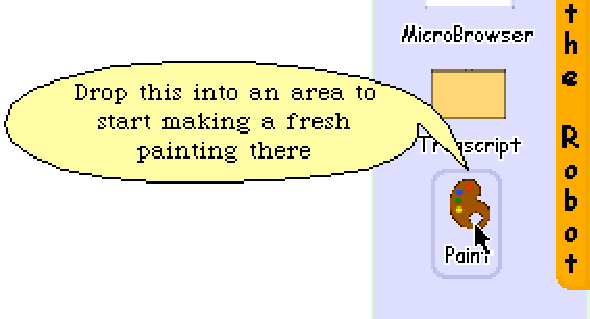
\includegraphics[width=6cm]{paintToolCaroFlap} 
\end{center}
\caption{ \label{fig:paintToolCaroFlap} Getting the painting editor from the blue flap.}
\end{figure}



%\begin{figure}
%\begin{center}
%\includegraphics[width=6cm]{widgetFlaps} \includegraphics[width=6cm]{paint}  
%\end{center}
%\caption{Left: The widget flap. \label{fig:Paint} Right: Getting the painting \replace{editor}{tool} from the widget flap. \label{fig:widgetFlap}}
%\end{figure}

%\begin{figure}
%\begin{center}
%\includegraphics[width=5cm]{gettingPaintEditor}
%\end{center}
%\caption{Getting the painting \replace{editor}{tool} from the object palette. \label{fig:gettingPaintEditor}}
%\end{figure}

\begin{figure}
\begin{center}
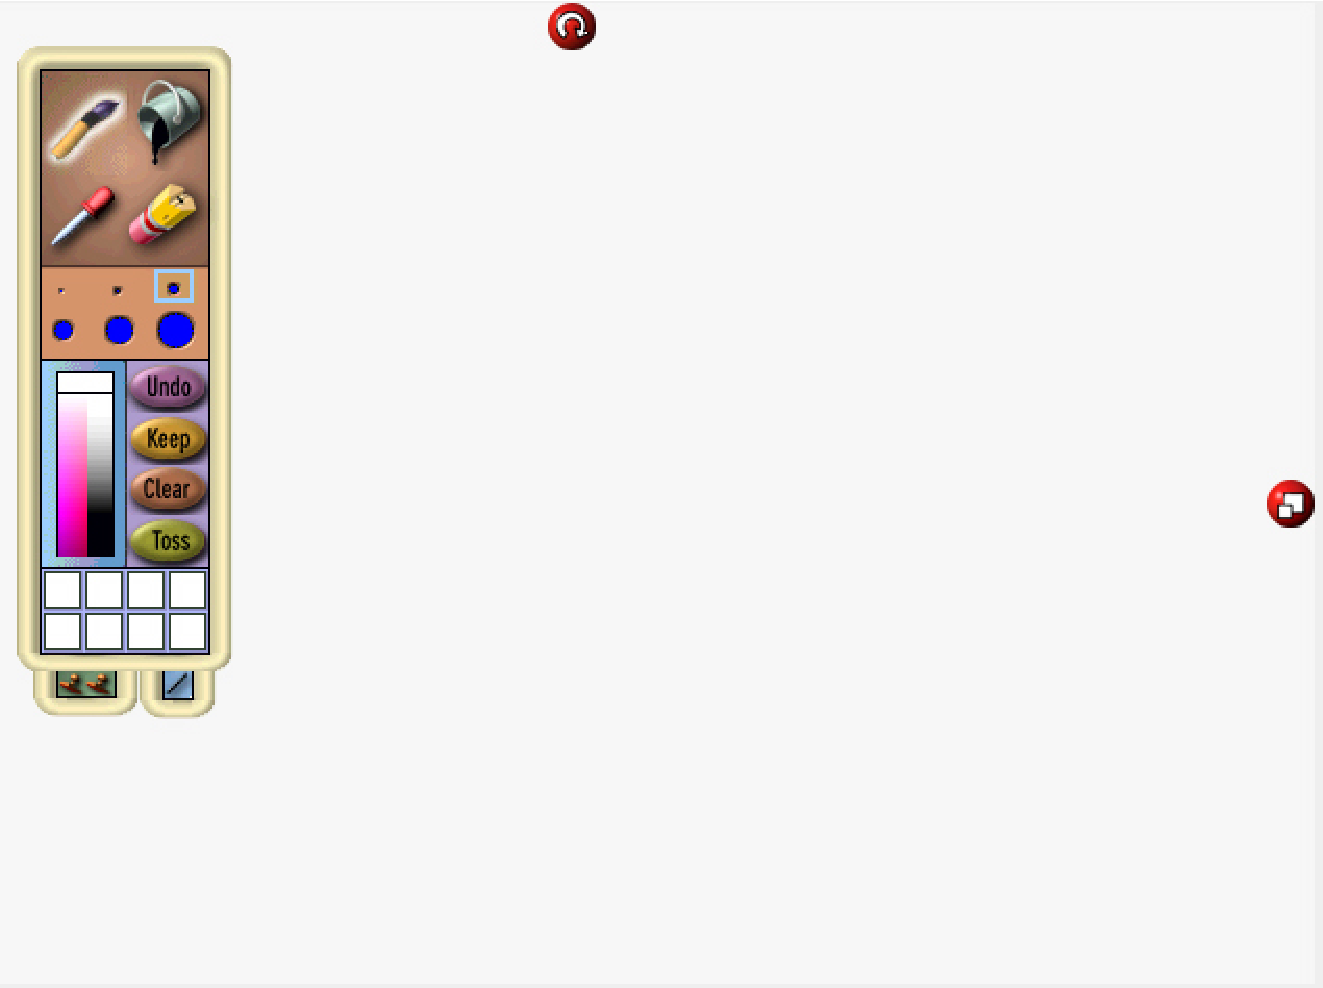
\includegraphics[width=14cm]{paintOpen}
\caption{The \add{opened} painting editor\remove{ opens}. \label{fig:paintOpen}}
\end{center}
\end{figure}

\paragraph{Step2. \replace{Drawing  a}{Draw the} New \replace{Graphics}{Graphic}. }
The second step is to draw a new \replace{graphics}{graphic} for \remove{representing} your robot. Draw your robot \replace{as if it would point towards}{pointing to} the right\add{,} as shown in Figure~\ref{fig:luth}. The painting editor has the usual \replace{facilities such as different}{features like choosing the} brush size, filling \add{a} region, \replace{selecting}{repeating a selected} region\remove{ as repeated pattern}, \add{and} selecting \add{the} painting color (see Figure~\ref{fig:palette}). The painting \replace{editor}{tool also} has two buttons \add{(}shown in Figure~\ref{fig:rotate}\add{)}  to rotate and zoom your drawing. 

\begin{figure}
\begin{center}
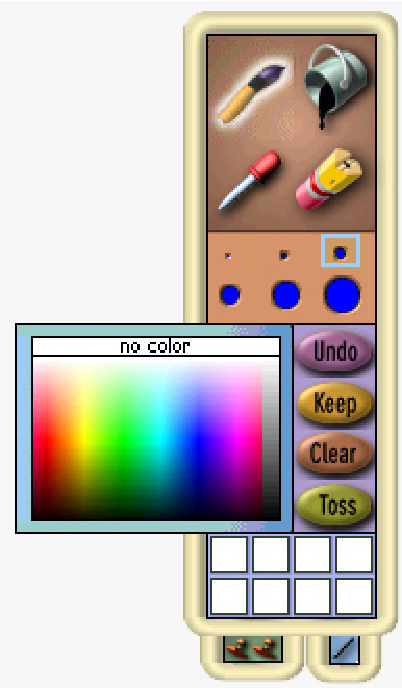
\includegraphics[width=5cm]{palette}
\end{center}
\caption{The painting \replace{editor's}{tool's color} palette. \label{fig:palette}}
\end{figure}

\begin{figure}
\begin{center}
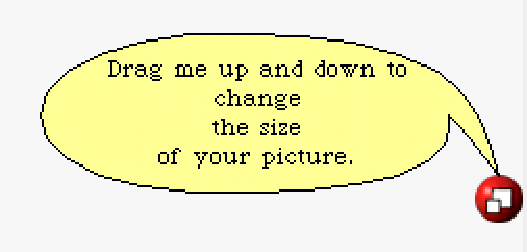
\includegraphics[width=5cm]{zoomButton} 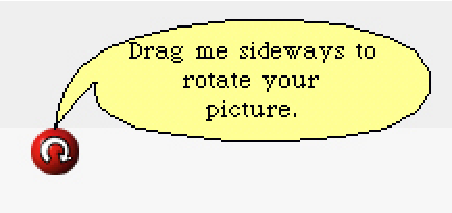
\includegraphics[width=5cm]{rotateButton}
\end{center}
\caption{The zoom and rotate buttons. \label{fig:zoom}\label{fig:rotate}}
\end{figure}


\begin{figure}
\begin{center}
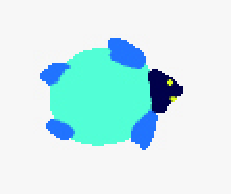
\includegraphics{luth} 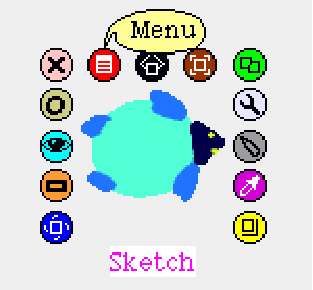
\includegraphics{debugMenu}
\end{center}
\caption{Left: Drawing a new shape pointing toward the east. \label{fig:luth} Right: \replace{Getting}{Picking} the red \add{halo for the graphic's} menu. \label{fig:redMenu}}
\end{figure}

\paragraph{Step3. Keeping the Graphics.} Once you are satisfied with your drawing, you \replace{should}{can} press the button \button{keep}. This closes the editor \replace{but let}{and leaves} your \replace{graphics}{graphic} on the screen. \replace{Now we have to}{Next,} associate the \replace{graphics}{graphic} with the \ct{\Turtle} class. To do \replace{so}{this} you \remove{should} bring \add{up} the halos on the \replace{graphics}{graphic} (\add{with the} Option \add{mouse} click), click on the red halo as shown in Figure~\ref{fig:redMenu} to pop up a menu, and select the menu item \textbf{keep as robot}.\add{\paragraph
} 
Now you are ready to see if your drawing 
\replace{fits well}{looks good on} your robot. 

\fprod{this section will change: @@keep as robot@@}
@@keep as robot@@
@@should change the keep to store it into the turtle@@

Execute \tscrref{scr:lookimage} and you should get a new robot with the shape you draw. Note that all the  robots that you \remove{will} create will be shown using the same \replace{graphics}{graphic}. But each of them can still be \replace{shown as}{changed to} a triangle or circle.


\begin{scriptwithtitle}{Use of \ct{lookLikeImage}}\label{scr:lookimage}
| \caro luth | 
luth := \Turtle new.
luth  lookLikeImage.
\caro := \Turtle new.
\caro lookLikeCircle.
\end{scriptwithtitle}

\summa
\begin{table}[h]
\centering
\begin{tabular}{||p{3cm}|p{4cm}|p{6.5cm}||} \hline
% after \\ : \hline or \cline{col1-col2} \cline{col3-col4} ...
Method&Description&Example\\[1ex] \hline
\ct{lookLikeCircle}&Change the shape of the receiver to \remove{be} a circle& \ct{\Turtle new lookLikeCircle}\\ \hline
\ct{lookLikeTriangle}&Change the shape of the receiver to \remove{be} a triangle&\ct{\Turtle new lookLikeTriangle}\\ \hline
\ct{lookLikeImage}&Change the \replace{appareance}{appearance} of the receiver to \remove{be as} the \replace{sketch}{graphic} you \replace{paint}{painted}& \ct{\Turtle new lookLikeImage} \\ \hline

\ct{penColor: aColor}&Change the color of the pen& \ct{\Turtle new penColor: Color blue}\\ \hline
\ct{penSize: aNumber}&Change the size of the pen. The default size is 1.&\ct{\Turtle new penSize: 3}\\ \hline

\ct{color: aColor}&Change the color of the receiver to the specified color& \ct{\Turtle new color: Color yellow}\\ \hline
\ct{extent: aPoint}&Change the size of the receiver. aPoint (w@h) specifies the new size of the receiver as the size of the rectangle. The first number is the width and the second the height. &\ct{\Turtle new extent: 80@100}\\ \hline

\end{tabular}
\end{table}

\ifx\wholebook\relax\else\end{document}\fi